%FIT
The Finite Integration Technique (\textbf{FIT}), which was introduced at 1976 by Thomas Weiland\cite{FIT_discrete_method} to solving the electromagnetical problems, is a numerical simulation method to discretize the integral form of fundamental Maxwell's functions.\\

The first thought of the \textbf{FIT} is to discretize the calculating volume. There is lot of methods to accomplish this mission. One common way is as Fig. \ref{fig:discretization_material} to discetize a brick-shape object into a \textbf{Cartesian Grid} (primary grid \textbf{G}). It is also possible to construct grid volume in cylinder coordinate or any other types of  coordinates\cite{FIT_triangular_discretization,FDTD_nonorthogonal_grids} for simplifying the calculation depending on dimensions of the object. In general  the computational grid is indicated as \\
\begin{align}
G=
(u(i),v(j),w(k))\in \mathbb{R}^3|&u(1)\leq u(i)\leq u(I),\nonumber\\
													 &v(1)\leq v(j)\leq v(J),\nonumber\\ 
													 &w(1)\leq w(k)\leq w(K)\quad \text{.}
\label{eq:grid}
\end{align}

$u(i)$,$v(j)$,$w(k)$ can be three components of any 3D coordinate systems. In following discussion all computations base on \textbf{Cartesian Coordinate system}.\\
%fig: discretization of the material
\begin{figure}[!ht]
\centering
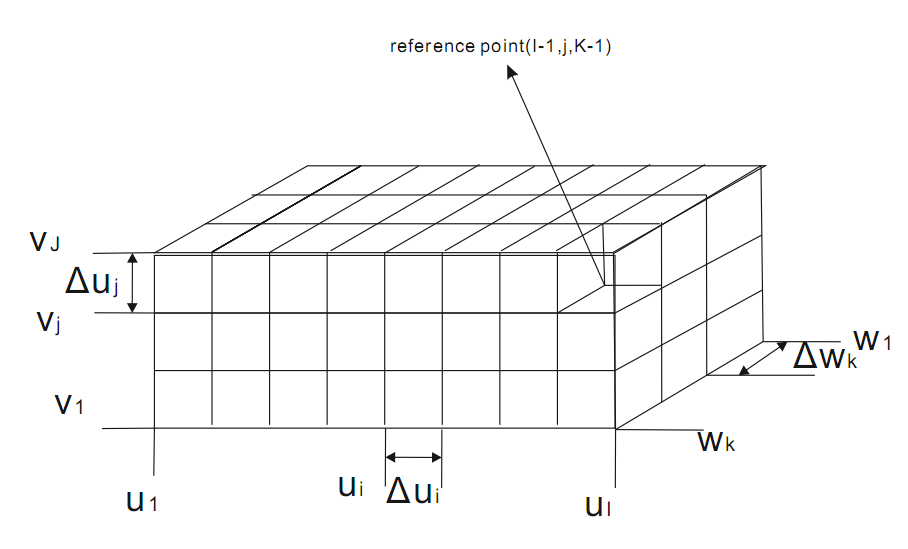
\includegraphics[width=0.8\textwidth]{bilder/grid_volum}
\caption{A Cartesian descretized Grid Volum\cite{script_FeldSim}.}
\label{fig:discretization_material}
\end{figure}
For calculations following primary elements are defined in \cite{script_FeldSim}:
\begin{itemize}
\item Points $P(i,j,k)$
\item Elemental Edge
    \begin{align*}
		\Delta u(i)&=\overline{u(i)u(i+1)}  \quad \mathrm{with}  \quad 1\leq i \leq I-1, \nonumber\\
		\Delta v(j)&=\overline{v(j)v(j+1)}  \quad \mathrm{with}  \quad 1\leq j \leq J-1, \nonumber\\
		\Delta w(k)&=\overline{w(k)w(k+1)}  \quad \mathrm{with}  \quad 1\leq k \leq K-1
		%\label{eq:discrete_edge}
		\end{align*}
\item Elemental Planes
		\begin{align*}
		A_{u}(j,k)&=\Delta v(j)\Delta w(k) \quad \mathrm{with}  \quad 1\leq i \leq I-1,1\leq j \leq J-1\nonumber\\
		&A_{v}(i,k),A_{w}(i,j)  \quad \mathrm{analogous}
		%\label{eq:discrete_plane}
		\end{align*}
\item Elemental Cells
		\begin{align*}
		V(i,j,k)=\Delta u(i)\Delta v(j)\Delta w(k)  \quad with  &\quad 1\leq i\leq I-1,\nonumber\\
		&1\leq j\leq J-1,\nonumber\\
		&1\leq k\leq K-1
		%\label{eq:discrete_cell}
		\end{align*}
\end{itemize}
A new index system has been introduced for numerical convenience:

\begin{equation}
n=1+(i-1)\cdot M_{u}+(j-1)\cdot M_{v}+(k-1)\cdot M{w}
\label{eq:discrete_index}
\end{equation}
Where $M_{u}=1,M_{v}=I,M_{w}=I\cdot J$. We can reindex primary elements with new index rules $n$ as following:
\begin{itemize}
\item Points $P(n) \quad \mathrm{with} \quad 1\leq n \leq N_{p}$
\item Elemental Edge
%$\delta u(i)=\overline{u(i)u(i+1)} with 1\leq{i}\leq{I-1},$
    \begin{align*}
		\Delta u(n)&=\overline{u(n)u(n+1)}  \quad \mathrm{with} \quad 1\leq n \leq N_{p}, \nonumber\\
		\Delta v(n)&=\overline{v(n)v(n+1)}  \quad \mathrm{with} \quad 1\leq n \leq N_{p}, \nonumber\\
		\Delta w(n)&=\overline{w(n)w(n+1)}  \quad \mathrm{with} \quad 1\leq n \leq N_{p}
		%\label{eq:discrete_edge_n}
		\end{align*}
\item Elemental Planes
		\begin{align*}
		A_{u}(n)&=\Delta v(n)\Delta w(n) \quad \mathrm{with} \quad 1\leq n\leq N_{p}\nonumber\\
		&A_{v}(n),A_{w}(n)  \quad \mathrm{analogous}
		%\label{eq:discrete_plane_n}
		\end{align*}
\item Elemental Cells
		\begin{equation*}
		V(n)=\Delta u(n)\Delta v(n)\Delta w(n)  \quad \mathrm{with} \quad 1\leq n\leq N_{p}
		%\label{eq:discrete_cell_n}
		\end{equation*}
\end{itemize}
Where $N_{p}$ is the total number of the grid points:
\begin{equation*}
N_{p}=I\cdot J\cdot K
%\label{eq:np}
\end{equation*}

The next step is to discretize Maxwell's equations in their integral form (\ref{eq:maxwell_1}-\ref{eq:maxwell_4}) 
\begin{align}
\oint_{\partial A}\vec{E}\cdot\mathrm{d}\vec{s}&=
-\frac{\mathrm{d}}{\mathrm{d}t}\int_{A}\vec{B}\cdot\mathrm{d}\vec{A}
\label{eq:maxwell_1}\\
\oint_{\partial A}\vec{H}\cdot\mathrm{d}\vec{s}&=
\int_{A}(\frac{\partial\vec{D}}{\partial t}+\vec{J})\cdot\mathrm{d}\vec{A}
\label{eq:maxwell_2}\\
\oint_{\partial V}\vec{D}\cdot\mathrm{d}\vec{A}&=
\int_{V}\rho\mathrm{d}V
\label{eq:maxwell_3}\\
\oint_{\partial V}\vec{B}\cdot\mathrm{d}\vec{A}&=0
\label{eq:maxwell_4}
\end{align}
and additional equations (\ref{eq:maxwell_5}-\ref{eq:maxwell_7}).:
\begin{align}
\vec{D}&=\epsilon_{0}\epsilon_{r}\vec{E}
\label{eq:maxwell_5}\\
\vec{B}&=\mu_{0}\mu_{r}\vec{H}
\label{eq:maxwell_6}\\
\vec{J}&=\kappa\vec{E}+\vec{J_{s}}
\label{eq:maxwell_7}
\end{align}
